\documentclass[11pt]{article}

\usepackage{a4wide}
\usepackage[utf8]{inputenc}
\usepackage[russian]{babel}
\usepackage{graphicx}
\usepackage{indentfirst} 
\usepackage{amsmath}
\usepackage{amssymb}
\usepackage{amsthm}
\usepackage{floatflt}
\usepackage{multicol}

\newtheorem{Th}{Теорема}

\newcommand\Real{\mathbb{R}} 
\newcommand\PS{\mathcal{P}}
\newcommand\X{\mathcal{X}} 
\newcommand\Sup[2]{\rho( #1 \, | \, #2 )}
\newcommand\Cl[2]{\begin{bmatrix}
#1 \\ #2
\end{bmatrix}}
\newcommand\Conv[1]{{\rm conv}\left\{ #1 \right\}}
\newcommand\Sgn{{\rm sgn \,}}
\DeclareMathOperator*{\Argmax}{Argmax}
\DeclareMathOperator{\Ker}{Ker}
\DeclareMathOperator{\Arccos}{arccos}


\begin{document}

\thispagestyle{empty}

\begin{center}
\ \vspace{-3cm}


\includegraphics[width=0.5\textwidth]{msu.eps}\\
{\scshape Московский государственный университет имени М.~В.~Ломоносова}\\
Факультет вычислительной математики и кибернетики\\
Кафедра системного анализа

\vfill

{\LARGE Отчёт по самому важному предмету}

\vspace{1cm}

{\Huge\bfseries <<Задание 1 практикума по оптимальному управлению>>}
\end{center}

\vspace{1cm}

\begin{flushright}
  \large
  \textit{Студент 315 группы}\\
  Д.\,М.~Сотников

  \vspace{5mm}

  \textit{Руководитель практикума}\\
  к.ф.-м.н., доцент П.\,А.~Точилин
\end{flushright}

\vfill

\begin{center}
Москва, 2020
\end{center}

\newpage
\part{Теоретическая часть}
\section{Постановка задачи}

Дана система обыкновенных дифференциальных уравнений
\[
\dot{x}\left (t\right ) = A x\left (t\right ) + B u\left (t\right ) + f, \quad t \in [t_0, +\infty),
\]
где $x(t) \in \Real^2, \ u(t) \in \Real^2, \ A \in \Real^{2 \times 2}, \ B \in \Real^{2 \times 2},
 \ f \in \Real^2$, а значения функции управления $u(t) \in \PS \quad \forall t \in [t_0, +\infty)$.

Множество допустимых управлений имеет вид 
$$ \PS = \left\{ x \in \Real^2 \colon \ x_1^2 + a x_2^2 \leq b, \ ax_1^2 + x_2^2 \leq b \right\}, \quad a,b > 0.$$
Будем считать, что $a > 1$, в противном случае сделаем замену $a = \frac{1}{a}, \ b = \frac{b}{a}$.

Начальное множество зачений фазового вектора: $$\X_0 = \mathbb{B}(x_0, r_0).$$

Терминальное множество: $$\X_1 = \Conv{x_1^{\left(1\right)}, \ldots, x_1^{\left(n\right)}} + \mathbb{B}(0, \epsilon), \quad n \in \mathbb{N}.$$

Необходимо численно решить задачу быстродействия, то есть перевести систему из множества $\X_0$ в множество $\X_1$,
минимизируя время перемещения $(t_1 - t_0)$. При этом, поскольку система является линейной и автономной, будем считать, что $t_0 = 0$.


\section{Принцип максимума Понтрягина}
Решение задачи опирается на принцип максимума Понтрягина для линейных систем~\cite{rublev}.
\begin{Th}[Принцип максимума Понтрягина] \label{PMP}
Пусть $(x^*(\cdot), \ u^*(\cdot))$ --- оптимальная пара, $t_1^*$ --- соответствующее ей время перемещения. Тогда существует дифференцируемая функция 
$\psi(\cdot) \not\equiv 0$, для которой выполнено
\begin{enumerate}
\item $\langle \psi(t), \ Bu^*(t) \rangle = \Sup{\psi(t)}{B \PS}$ для почти всех $t \in [0, t_1^*]$; 
\item $\langle \psi(0), \ x^*(0) \rangle = \Sup{\psi(0)}{\X_0}$;
\item $\langle -\psi(t_1^*), x^*(t_1^*) \rangle = \Sup{-\psi(t_1^*)}{\X_1}$.
\end{enumerate}
При этом функция $\psi(\cdot)$ является решением сопряженной системы $\dot \psi(t) = -A^T\psi(t)$, а
класс управлений представляет собой множество измеримых функций, принимающих значения в $\PS$.
\end{Th}
 
Заметим, что если $\psi(\cdot)$ удовлетворяет условиям теоремы, то им будет удовлетворять и функция 
$\alpha \psi(\cdot), \ \forall \alpha > 0$. Это следует из линейности скалярного произведения и 
положительной однородности опорной функции. Поэтому можно считать, что $\|\psi(0)\| = 1$.

Перебирая по единичному кругу параметр $\psi(0) = \psi^0$, можно найти все возможные траектории 
и управления, удовлетворяющие принципу максимума Понтрягина, что существенно
сузит класс функций, среди которых следует искать решение. Оптимальная при этом 
имеет наименьшее значение функцинала $t_1$.

Для проверки пунктов теоремы необходимо знать опорные функции и векторы множеств $\X_0, \ \X_1, \ \PS$, 
которые можно найти аналитически.

\section{Вычисление опорных функций и множеств}
В этом разделе приведено аналитическое вычисление опорных функций для начального, терминального множества и множества допустимых управлений.

Поскольку $\X_0$ является шаром, его опорная функция известна и имеет вид
$$\Sup{l}{\X_0} = \Sup{l}{\left\{x_0\right\}} + \Sup{l}{\mathbb{B}(0, r_0)} = 
\langle l, \ x_0 \rangle + r_0\|l\|.$$
Это значение достигается на опорном векторе 
$$x^* = x_0 + \frac{l}{\|l\|}r_0.$$

Для вычисления опорной функции $X_1$ воспользуемся свойством линейности $\rho$ по второму аргументу и 
тем, что опорная функция для выпуклой комбнации точек является максимумом скалярных произведений
вектора $l$ на эти точки:
$$\Sup{l}{\X_1} = \Sup{l}{\Conv{x_1^{\left(1\right)},, \ldots, x_1^{\left(n\right)}}} + \Sup{l}{\mathbb{B}(0, \epsilon)} =
\max_{i = 1,\ldots,n} \langle l, \ x_1^{\left(i\right)} \rangle + \epsilon \|l\|.$$

Множество всех опорных векторов $X^*$ для $\X_1$ есть сумма опорных множеств для 
$\Conv{x_1^{\left(1\right)},, \ldots, x_1^{\left(n\right)}}$ и $\mathbb{B}(0, \epsilon)$, и поэтому
имеет вид
$$ X^* = \Argmax_{x_1^{\left(i\right)}, \ i = 1, \ldots, n} \langle l, \ x_1^{\left(i\right)}\rangle + \frac{l}{\|l\|
}\epsilon.$$
При этом $\Argmax\limits_{x_1^{\left(i\right)}, \ i = 1, \ldots, n} \langle l, \ x_1^{\left(i\right)}\rangle$ состоит из одной точки
--- вершины многоугольника --- в случае, когда $l$ не перпендикулярен ни одной из сторон, или 
содержит всю соответствующую сторону в противном случае.

Множество $\PS$ является пересечением двух эллипсоидов \\
$$x_1^2 + a x_2^2 \leq b,$$
$$ax_1^2 + x_2^2 \leq b,$$
где $a > 1, \ b > 0$. \\

\noindent
\parbox[b][5cm][t]{50mm}{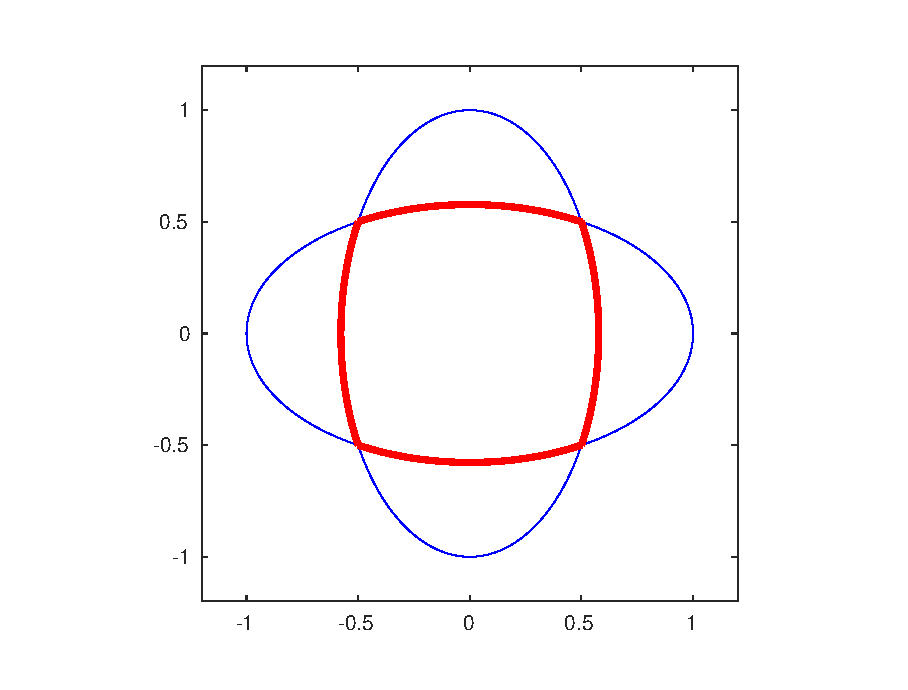
\includegraphics[height=50mm]{P_set.eps}}
\hfill
\parbox[b][5cm][t]{90mm}{
На рисунке множество $\PS$ отмечено красным. Заметим, что, в силу симметрии, достаточно найти опорную
функцию и опорный вектор только в случае $l_1 > l_2 > 0$.

Используя функцию Лагранжа, находим условный экстремум на эллипсе $x_1^2 + a x_2^2 = b$:
$$x_1^* = \sqrt{\frac{b}{a}}\frac{l_1}{\sqrt{l_1^2+al_2^2}}, \ x_2^* = \frac{l_2\sqrt{ab}}{\sqrt{l_1^2+al_2^2}}.$$
}

Найденные решения являются опорными векторами только в том случае, когда лежат на $\partial \PS$, 
а именно когда $|x_2^*| < \sqrt{\frac{b}{a+1}}$. Опорная функция при это принимает значение 
$\sqrt{\frac{b}{a}}\sqrt{l_1^2+al_2^2}$. В случае верхней и нижней стороны множества по аналогии получаем
$$\ x_1^* = \frac{l_1\sqrt{ab}}{\sqrt{al_1^2+l_2^2}},\  x_2^* = \sqrt{\frac{b}{a}}\frac{l_2}{\sqrt{al_1^2+l_2^2}}, \quad |x_1^*| < \sqrt{\frac{b}{a+1}}.$$
Опорная функция здесь равна $\sqrt{\frac{b}{a}}\sqrt{al_1^2+l_2^2}$. Во всех остальных случаях опорным 
вектором будет являться один из <<углов>> множества $\sqrt{\frac{b}{a+1}}[\Sgn{l_1}, \, \Sgn{l_2}]^T$.

Объединяя все вышесказанное, получаем итоговый вид для опорной функции:

\begin{equation}
\Sup{l}{\PS} = 
\left\{
	\begin{aligned}
	& \sqrt{\frac{b}{a}}\sqrt{l_1^2+al_2^2}, \ |l_1| > |l_2|, \  \frac{|l_2|\sqrt{ab}}{\sqrt{l_1^2+al_2^2}} < \sqrt{\frac{b}{a+1}},\\
	& \sqrt{\frac{b}{a}}\sqrt{al_1^2+l_2^2}, \ |l_2| > |l_1|, \  \frac{|l_1|\sqrt{ab}}{\sqrt{al_1^2+l_2^2}} < \sqrt{\frac{b}{a+1}},\\
	& \sqrt{\frac{b}{a+1}}(|l_1| + |l_2|), \ \text{иначе}.
	\end{aligned}	
\right.
\end{equation}

\newpage
\part{Практическая часть}
\setcounter{section}{0}
\section{Описание алгоритма}

Для поиска оптимальной траектории используется перебор по функциям, удовлетворяющим принципу
максимума, которые параметризованы одним числом --- углом вектора $\psi^0$, лежащего на 
единичной окружности.

Предполагается, что матрица $B$ является невырожденной, в противном случае будем добавлять к ней
незначительные случайные изменения до тех пор, пока ее определитель не станет больше некоторого
заданного числа $\epsilon_B$. Таким образом, $\Ker B = \{0\}$.

Отметим также, что сопряженная переменная $\psi(t) \not= 0, \quad \forall t \ge 0$.
 Это следует из единственности решения задачи Коши и требования $\psi(\cdot) \not\equiv 0$ 
 принципа максимума.

Ниже приведены шаги алгоритма вычисления субоптимальной пары.

\begin{itemize}
\item Создание равномерной сетки значений $\psi^0 = \psi(0)$ на окружности и численное решение
задачи Коши для сопряженной системы 

\begin{equation}
\left\{
	\begin{aligned}
	& \dot{\psi}(t) = -A^T\psi(t), \ t \in [0, 1], \\
	& \psi(0) = \psi^0
	\end{aligned}	
\right.
\end{equation}
с помощью функции ode45 на некоторой временной сетке.

\item В каждом узле сетки вычислим значение управления, пользуясь пунктом \textit{1.} принципа
 максимума: $u(t)$ является опорным вектором множества $\PS$ по направлению $B^T\psi(t) \not= 0$.
Опорный вектор этого множества был вычислен аналитически в прошлом разделе и определен однозначно.

\item Из условия трансверсальности \textit{2.} найдем начальную точку $x^0 = x(0)$ которая является
опорным вектором к $\X_0$ по направлению $\psi^0$ и также определена однозначно.

\item Зная начальное условие и управление, найдем траекторию $x[t]$, решая задачу Коши
\begin{equation}
\left\{
	\begin{aligned}
	& \dot{x}(t) = Ax(t) + Bu(t) + f, \ t \in [0, 1], \\
	& x(0) = x^0
	\end{aligned}	
\right.
\end{equation}

Получили, что каждому значению $\psi^0$ соответсвует единственная пара $(u(t), \ x(t))$, 
удовлетворяющая принципу максимума Понтрягина.
\item Численно проверим попадание траектории в терминальное множество, пользуясь свойством
\begin{equation}
x \in \X_1 \Leftrightarrow \langle l, \ x \rangle \le \Sup{l}{X_1}, \quad \forall l \colon \|l\| = 1.
\end{equation}

При попадании траектории в $\X_1$ установим значение $t_1^*$, далее которого вычисления других
 траекторий производиться не будут. Таким образом, к концу перебора $t_1^*$ будет равно минимальному
 времени перемещения для перебираемых траекторий, а соответствующая траектория, на которой достигается
 это значение, будет субоптимальной.
 
\item Если же ни одна из траекторий не попала в терминальное множество, продолжим их на отрезок
$[1, \, 2]$ и выполним аналогичные действия. Вычисления продолжаются до тех пор, пока $t \le t_{max}$,
где $t_{max}$ --- заранее задаванный параметр алгоритма. Если к этому времени ни одна из траекторий
не достигла $\X_1$, считаем, что задача не имеет решения.

\end{itemize}

\section{Проверка условия трансверсальности}
В описанном алгоритме никак не было задействовано условие трансверсальности \textit{3.} теоремы 
\ref{PMP}. Так как оптимальное управление удовлетворяет всем трем пунктам теоремы, найденное
решение также должно им удовлетворять, и пункт \textit{3.} можно использовать для оценки
погрешности (если условие трансверсальности не выполнено, найденное управление не может быть
оптимальным).

Для проверки данного условия необходимо найти опорную гиперплоскость в точке $x^1 \equiv x^*(t_1^*)$, 
где $x^*(\cdot)$ --- найденная субоптимальная траектория. Из гладкости границы $\partial \X_1$ 
следует, что
каждой его точке однозначно ставится в соответствие направление, по которому она
является опорным вектором. Таким образом для $x^1$
найдется единственный вектор $l$ такой, что $\langle l, \ x^1 \rangle = \Sup{l}{\X_1}, \ \|l\| = 1$.
Это вектор найдем численно с помощью сетки на единичной сфере, выбирая $l$, минимизирующий
 $|\langle l, \ x^1 \rangle - \Sup{l}{\X_1}|$. Если $l = \Cl{l_1}{l_2}$, то вектор нормали к опорной
 гиперплоскости имеет вид $n = \Cl{-l_2}{l_1}$. Для оценки <<неоптимальности>> найденного решения
 будем использовать угол $\alpha$ между $\frac{\psi(t_1^*)}{\|\psi(t_1^*)\|}$ и $n$, который можно
  найти по формуле $\alpha = \Arccos \langle \frac{\psi(t_1^*)}{\|\psi(t_1^*)\|}, \ n \rangle$.
  В случае идеального выполнения принципа максимума $\alpha = 0$.


\section{Локализация и уточнение вычислений}

При большой ошибке в условии трансверсальности \textit{3.} рассматривается более мелкая сетка для
параметра $\psi^0$, охватывающая меньший угол, чем на предыдущей итерации, и симметричная относительно
$\psi^0_*$ --- оптимального параметра на прошлой итерации.

Последовательное уточнение происходит до тех пор, пока ошибка в условии трансверсальности не 
станет достаточно маленькой.

\section{Примеры работы программы}

\paragraph{Пример 1\\}

\begin{equation}
A = \frac1{10}\begin{bmatrix}
1 & 0 \\ 1 & 1
\end{bmatrix},\ 
B = \begin{bmatrix}
10 & 0 \\ 0 & 10
\end{bmatrix}, \
f = \begin{bmatrix}
1 \\ 1
\end{bmatrix},
\end{equation}

$$\X_0 = \mathbb{B}\left(\Cl{-4}{7}, 1\right),$$
$$\X_1 = \Conv{\Cl{9}{3}, \Cl{7}{4}, \Cl{11}{5}, \Cl{10}{8}, \Cl{8}{8}} + \mathbb{B}(0, 1),$$
$$\PS = \{u\colon 2u_1^2 + u_2^2 \le 1, \ u_1^2 + 2u_2^2 \le 1 \}.$$

За одну итерацию работы программы значения функционала 
$$t_1^* = 1.1790,$$
а ошибка условия трансверсальности $\alpha = 0.0687^\circ$.

\begin{figure}[h]
\begin{multicols}{3}
	\hfill
	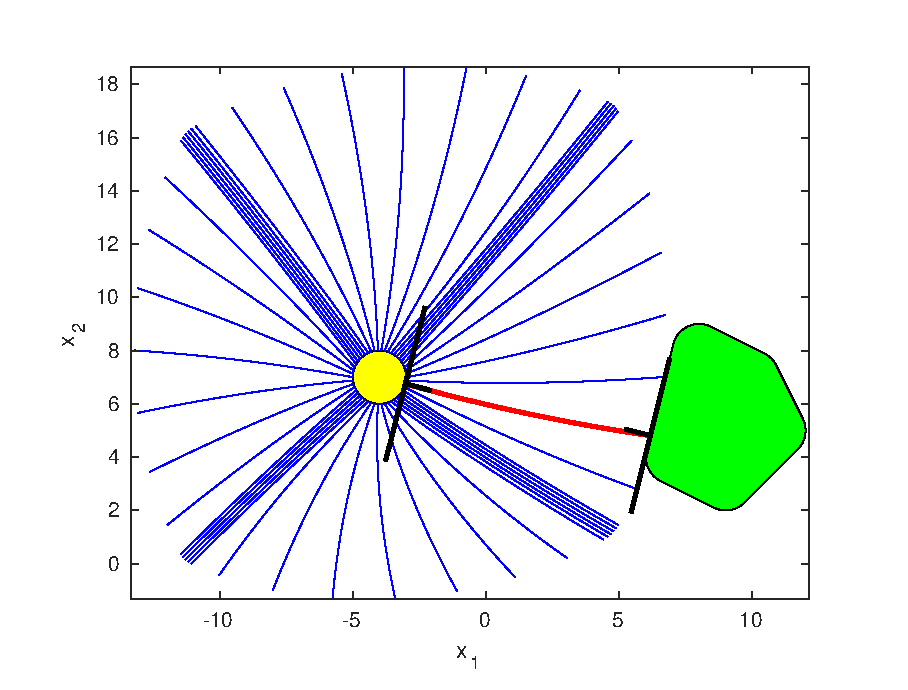
\includegraphics[width=45mm]{1xx.eps}
	\hfill
	\caption{График $(x_1, \, x_2)$}
	\hfill
	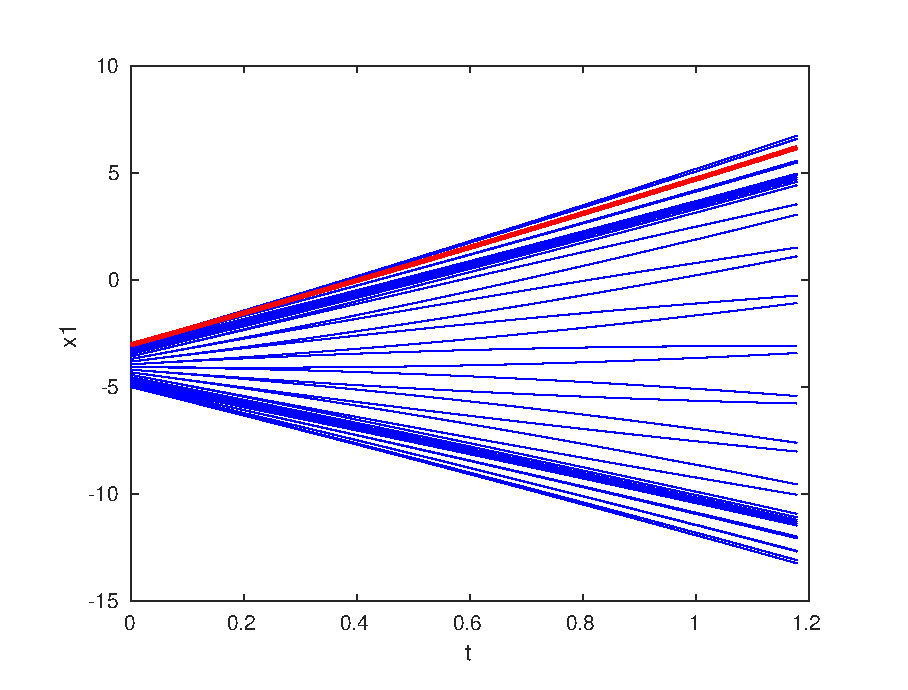
\includegraphics[width=45mm]{1tx1.eps}
	\hfill
	\caption{График $(t, \, x_1)$}
    \hfill
	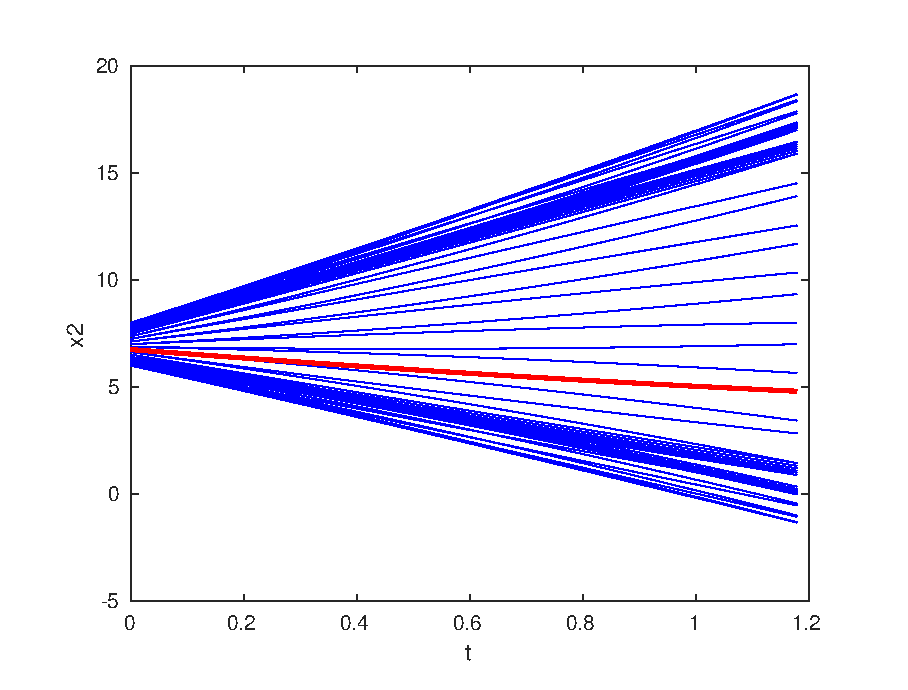
\includegraphics[width=45mm]{1tx2.eps}
	\hfill
	\caption{График $(t, \, x_2)$}
\end{multicols}

\begin{multicols}{3}
	\hfill
	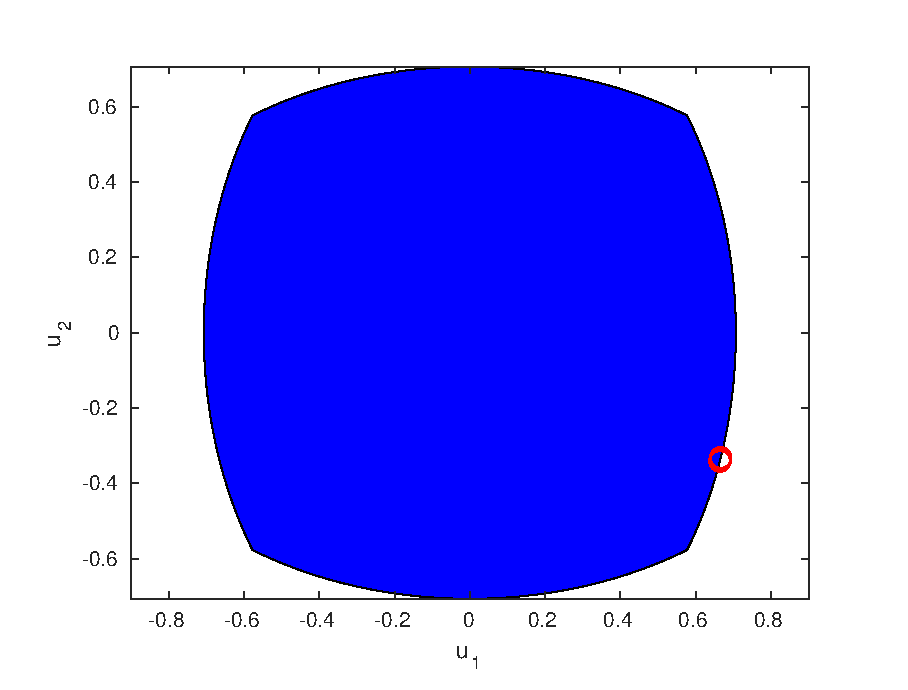
\includegraphics[width=45mm]{1uu.eps}
	\hfill
	\caption{График $(u_1, \, u_2)$}
	\hfill
	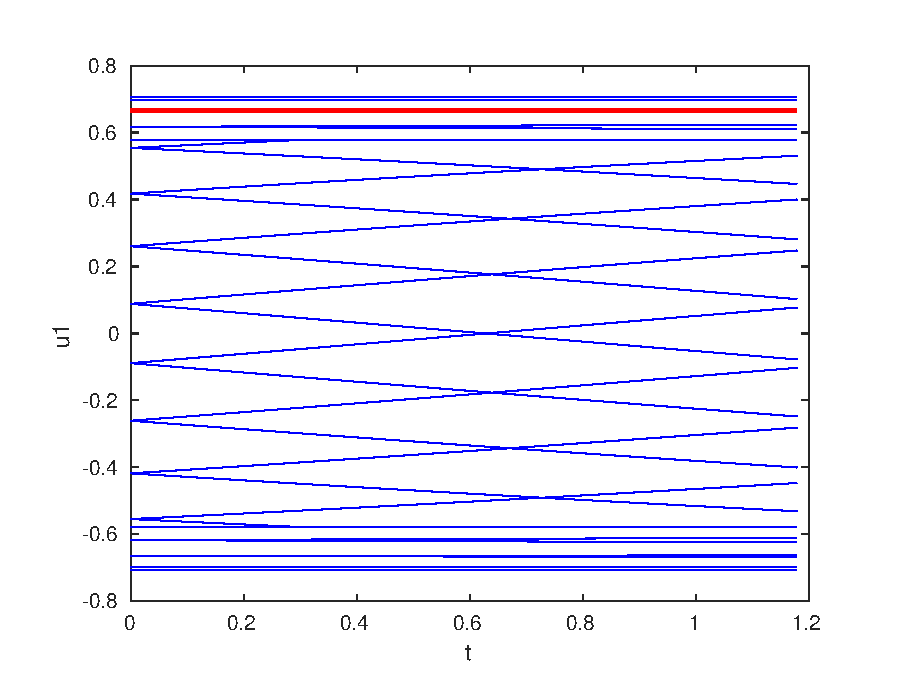
\includegraphics[width=45mm]{1tu1.eps}
	\hfill
	\caption{График $(t, \, u_1)$}
    \hfill
	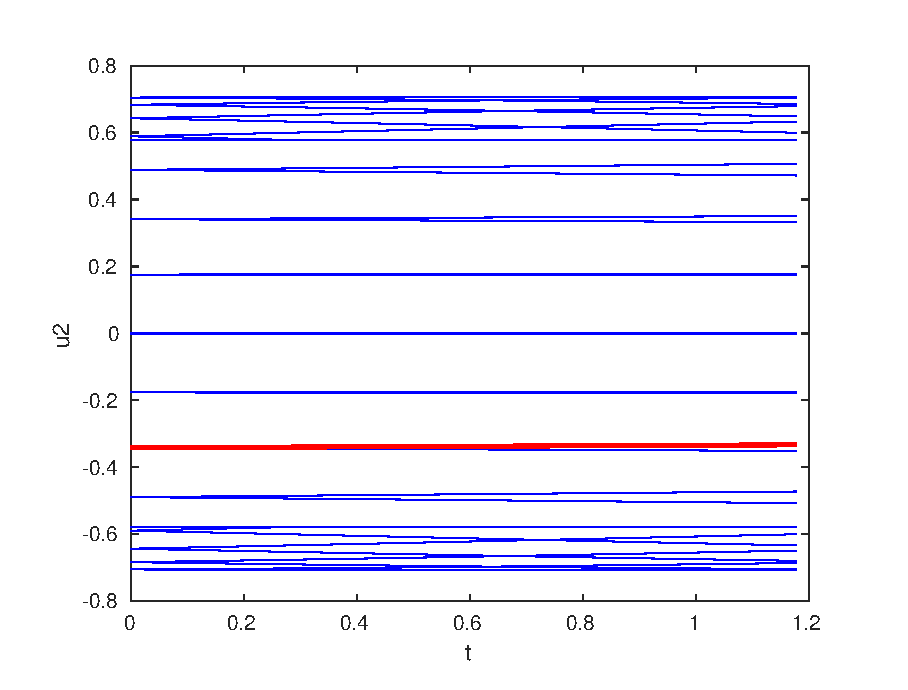
\includegraphics[width=45mm]{1tu2.eps}
	\hfill
	\caption{График $(t, \, u_2)$}
\end{multicols}

\begin{multicols}{3}
	\hfill
	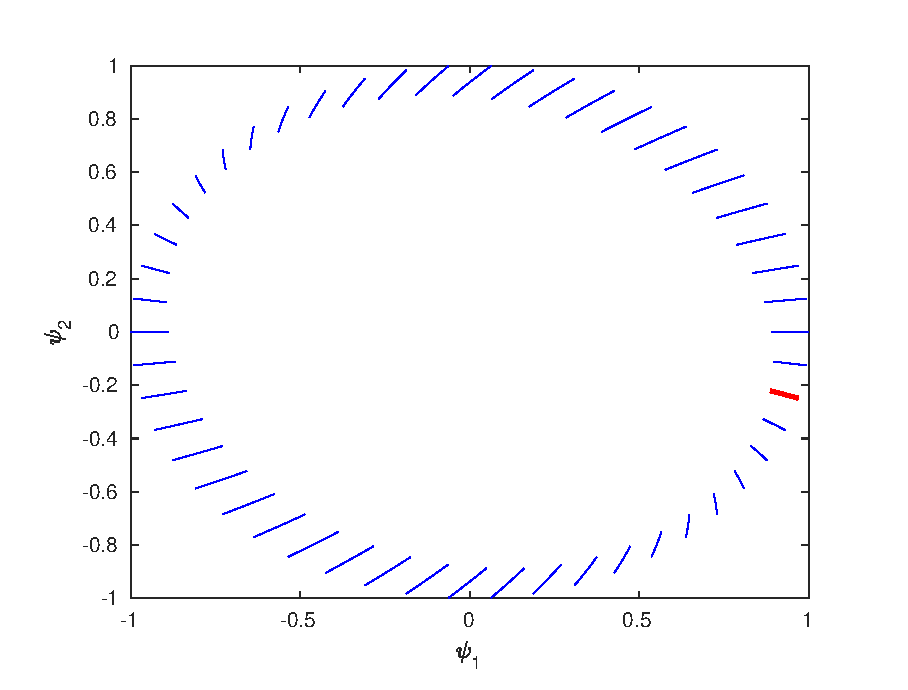
\includegraphics[width=45mm]{1pp.eps}
	\hfill
	\caption{График $(\psi_1, \, \psi_2)$}
	\hfill
	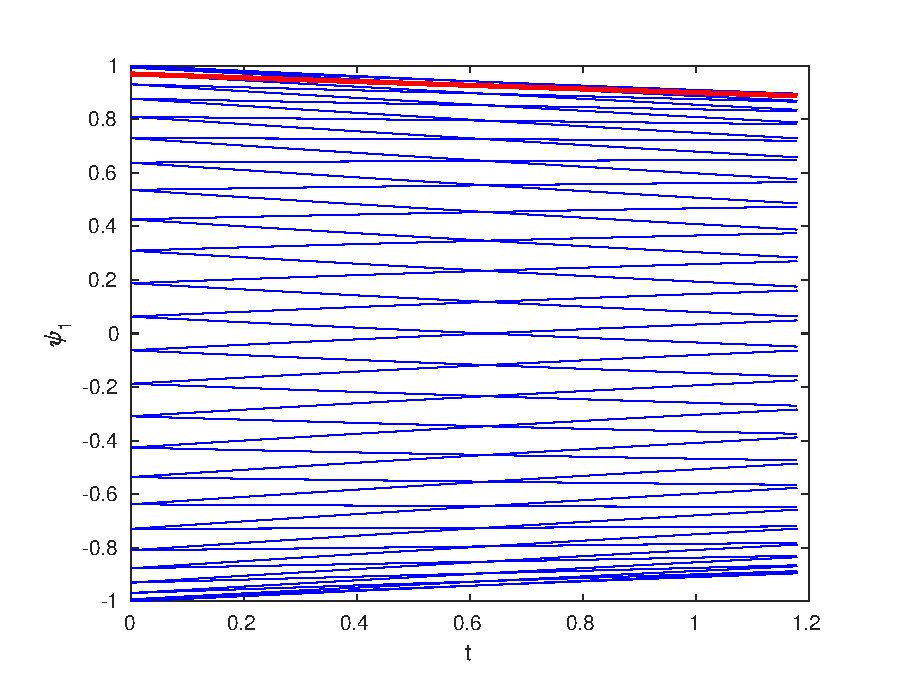
\includegraphics[width=45mm]{1tp1.eps}
	\hfill
	\caption{График $(t, \, \psi_1)$}
    \hfill
	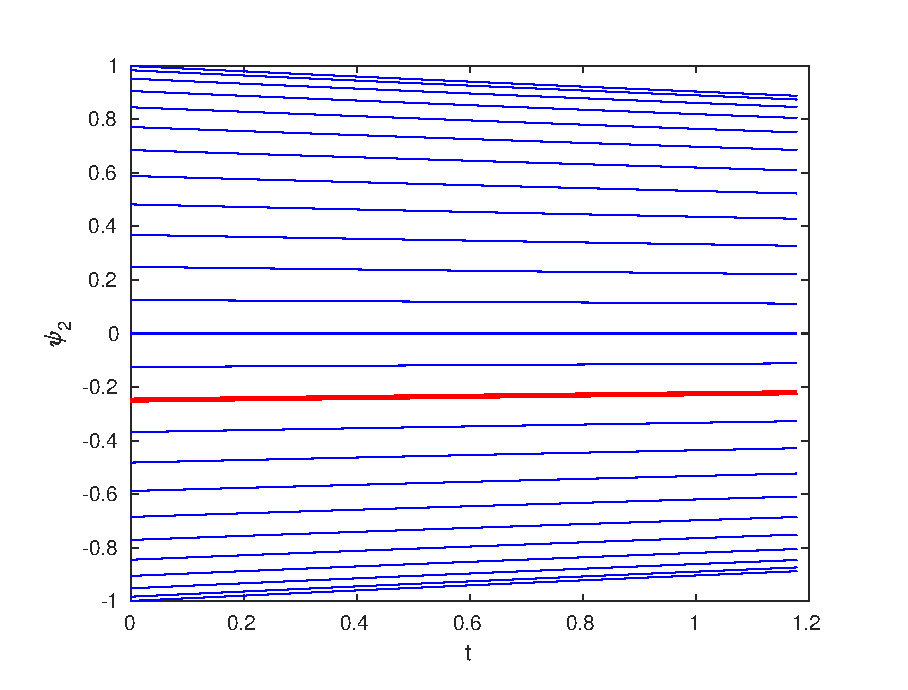
\includegraphics[width=45mm]{1tp2.eps}
	\hfill
	\caption{График $(t, \, \psi_2)$}
\end{multicols}
\end{figure}		

\newpage
\paragraph{Пример 2\\}
\begin{equation}
A = \frac1{10}\begin{bmatrix}
2 & -2 \\ 2 & 2
\end{bmatrix},\ 
B = \frac13\begin{bmatrix}
1 & 1 \\ 2 & 0
\end{bmatrix}, \
f = \begin{bmatrix}
0 \\ 0
\end{bmatrix},
\end{equation}

$$\X_0 = \mathbb{B}\left(\Cl{0}{-1}, 1\right),$$
$$\X_1 = \Conv{\Cl{0}{10}} + \mathbb{B}(0, 1),$$
$$\PS = \{u\colon u_1^2 + u_2^2 \le 1\}.$$


За одну итерацию работы программы значения функционала 
$$t_1^* = 1.0390,$$
а ошибка условия трансверсальности  $\alpha = 19.7232^\circ$.

\begin{center}
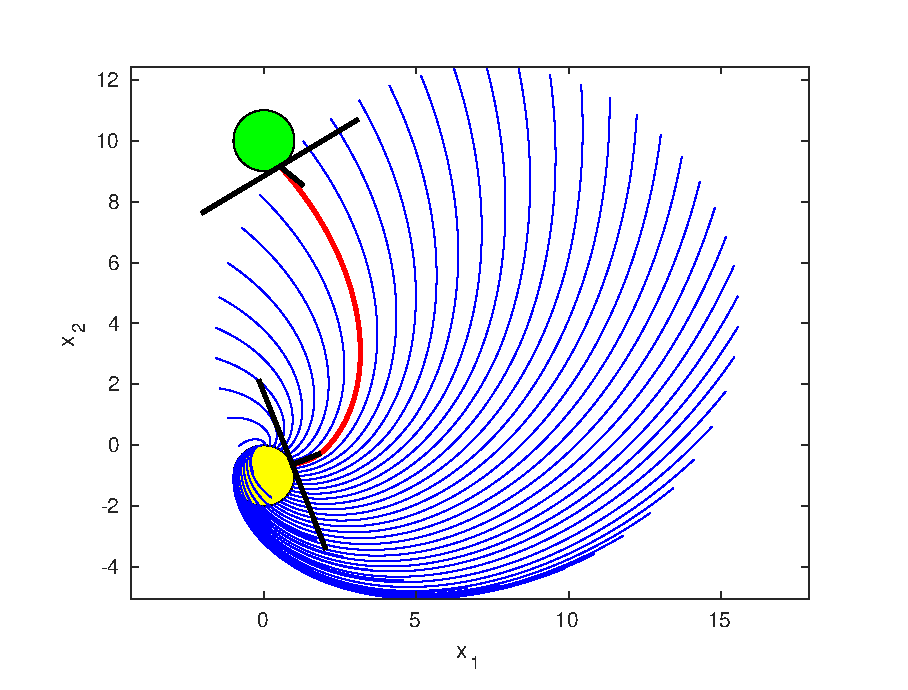
\includegraphics[width=90mm]{2xx_it1.eps}
\end{center}
 
После второй итерации
$$ t_1^* = 1.0370, $$
и ошибка $\alpha = 2.3975^\circ$.

\begin{figure}[h]
\begin{multicols}{3}
	\hfill
	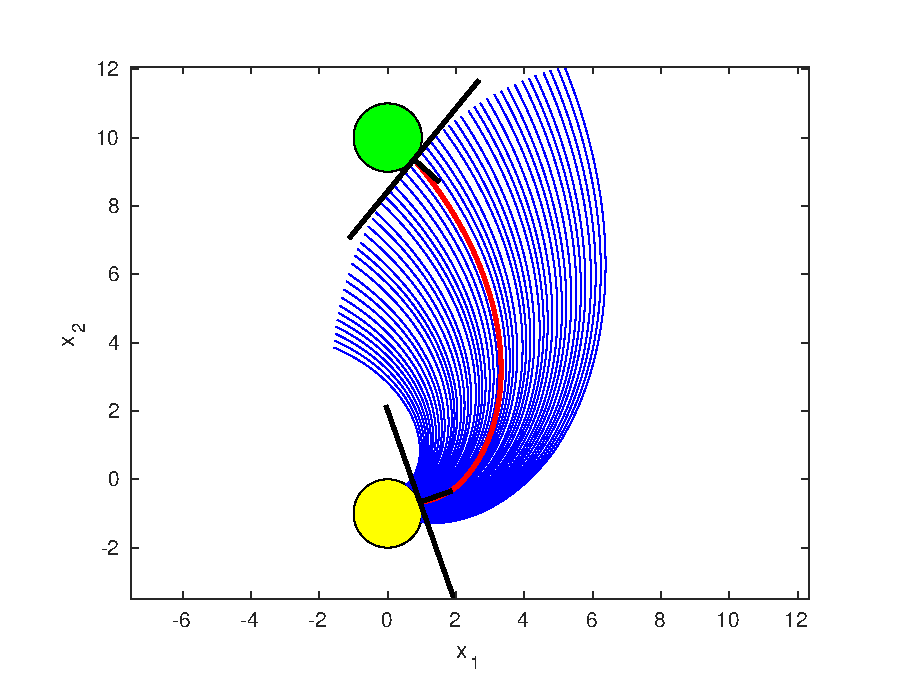
\includegraphics[width=45mm]{2xx.eps}
	\hfill
	\caption{График $(x_1, \, x_2)$}
	\hfill
	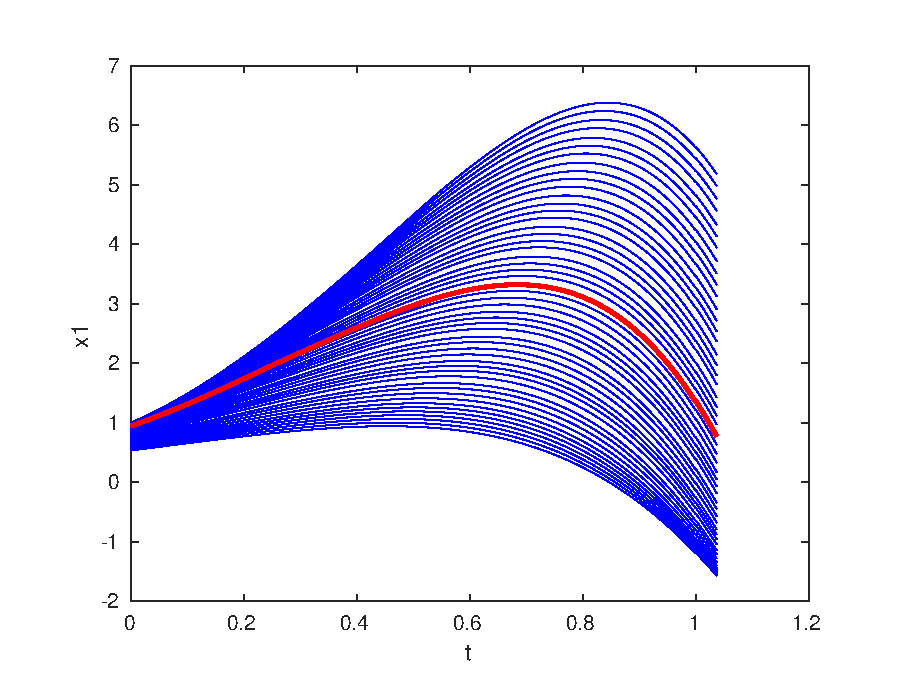
\includegraphics[width=45mm]{2tx1.eps}
	\hfill
	\caption{График $(t, \, x_1)$}
    \hfill
	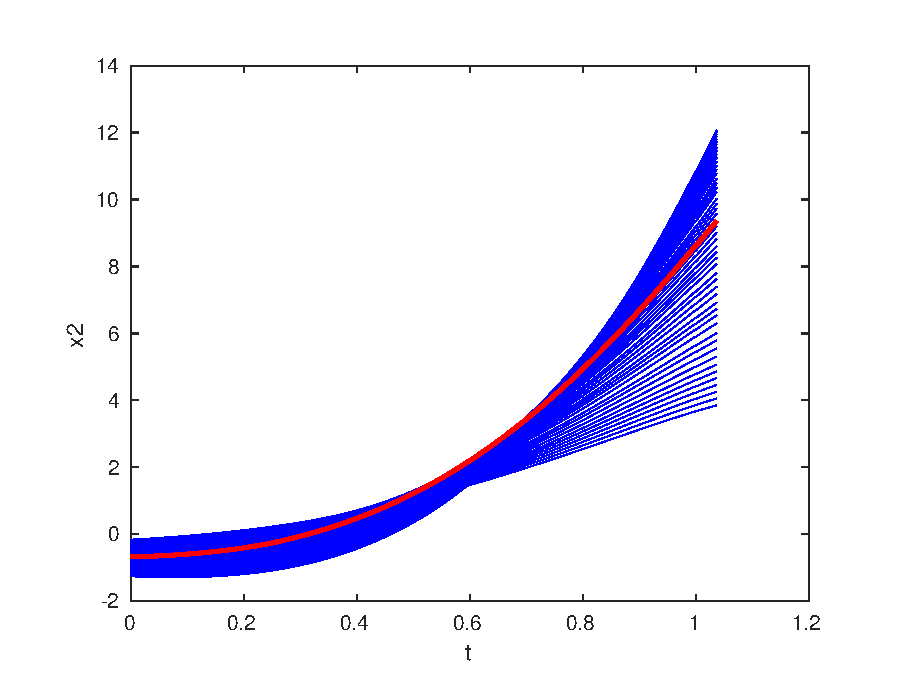
\includegraphics[width=45mm]{2tx2.eps}
	\hfill
	\caption{График $(t, \, x_2)$}
\end{multicols}

\begin{multicols}{3}
	\hfill
	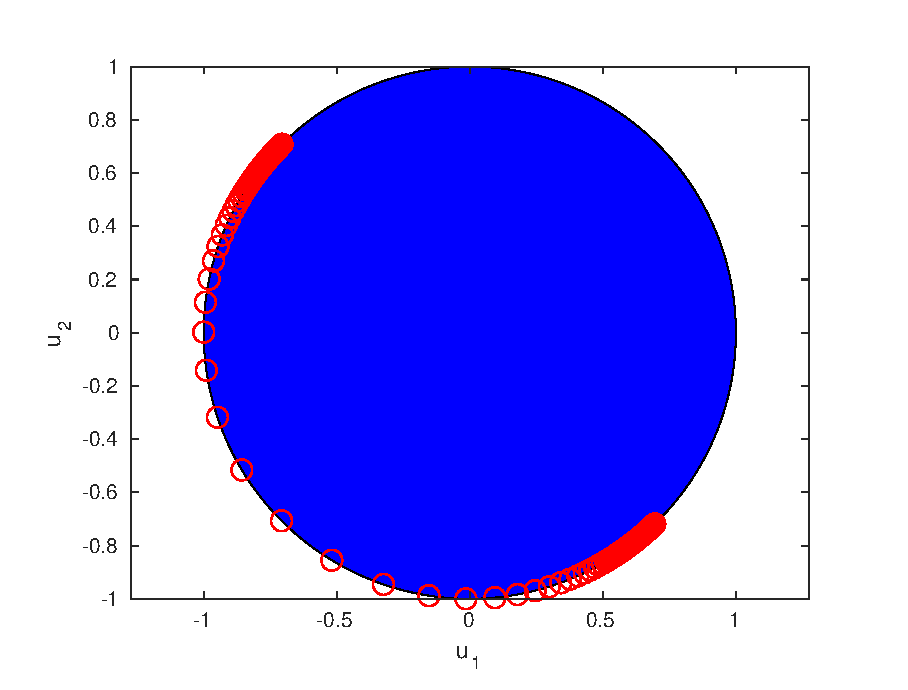
\includegraphics[width=45mm]{2uu.eps}
	\hfill
	\caption{График $(u_1, \, u_2)$}
	\hfill
	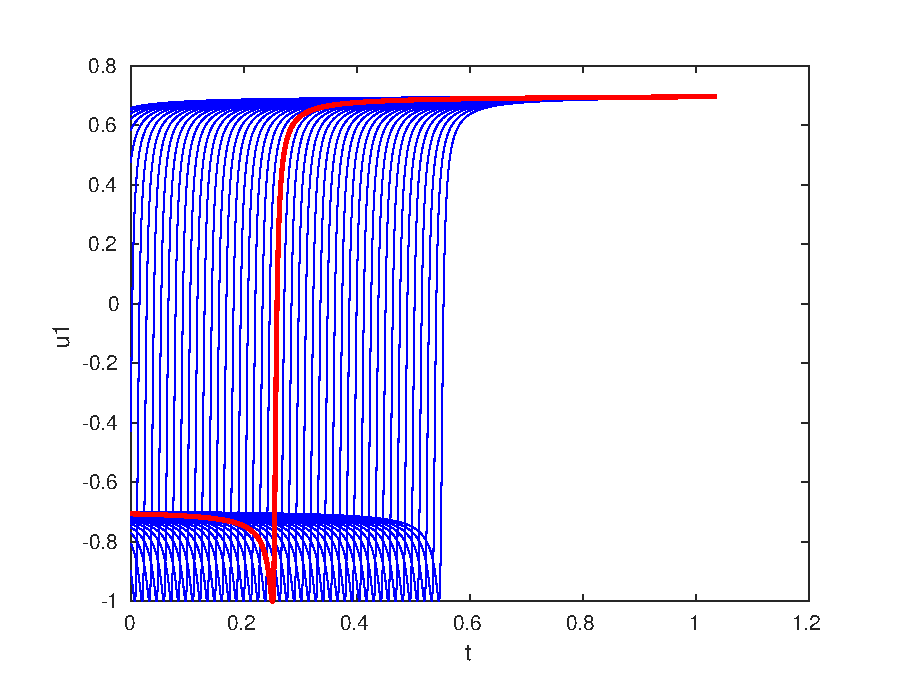
\includegraphics[width=45mm]{2tu1.eps}
	\hfill
	\caption{График $(t, \, u_1)$}
    \hfill
	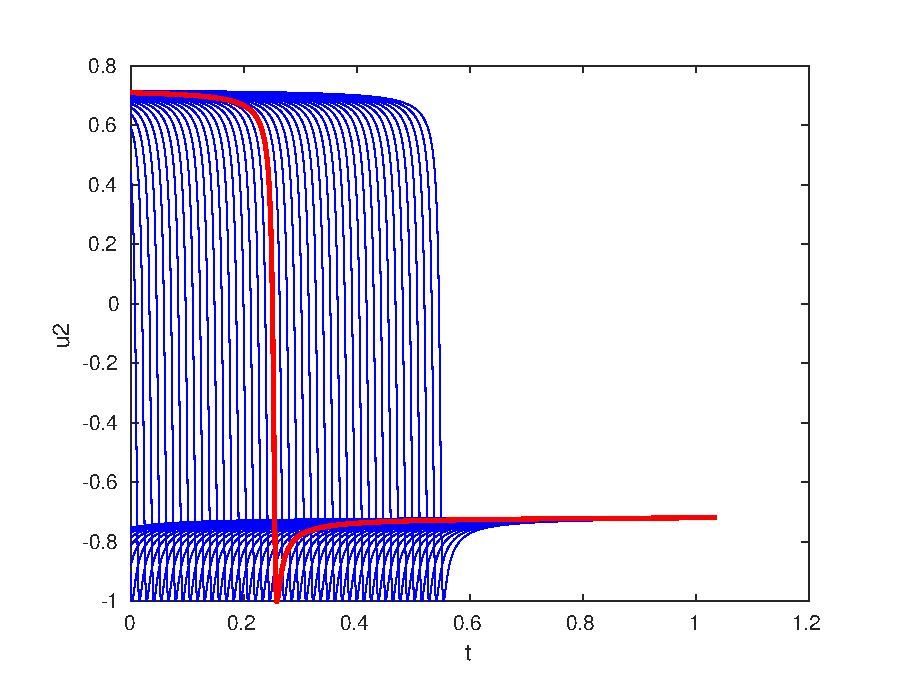
\includegraphics[width=45mm]{2tu2.eps}
	\hfill
	\caption{График $(t, \, u_2)$}
\end{multicols}

\begin{multicols}{3}
	\hfill
	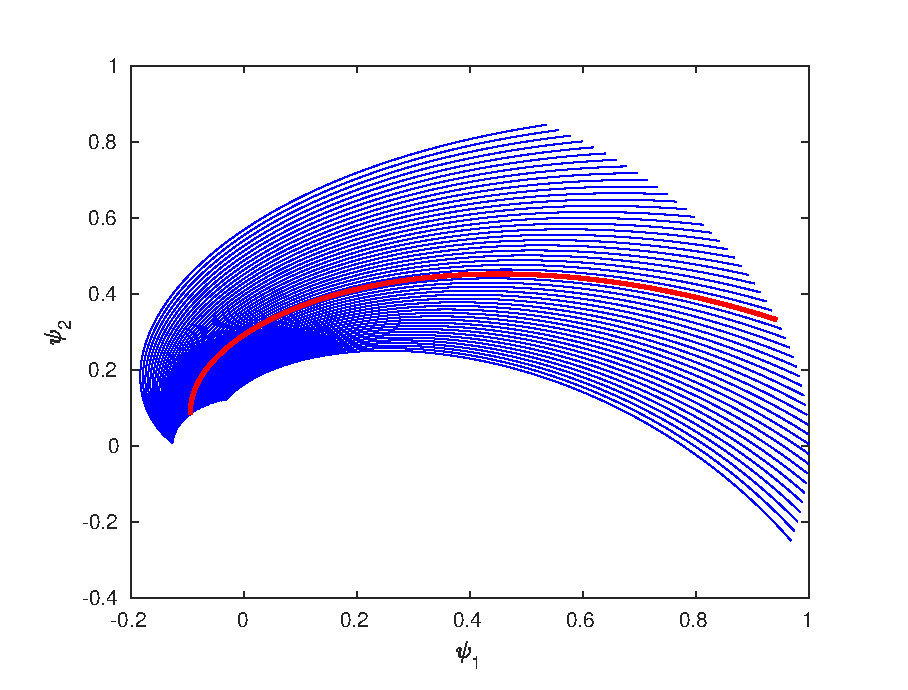
\includegraphics[width=45mm]{2pp.eps}
	\hfill
	\caption{График $(\psi_1, \, \psi_2)$}
	\hfill
	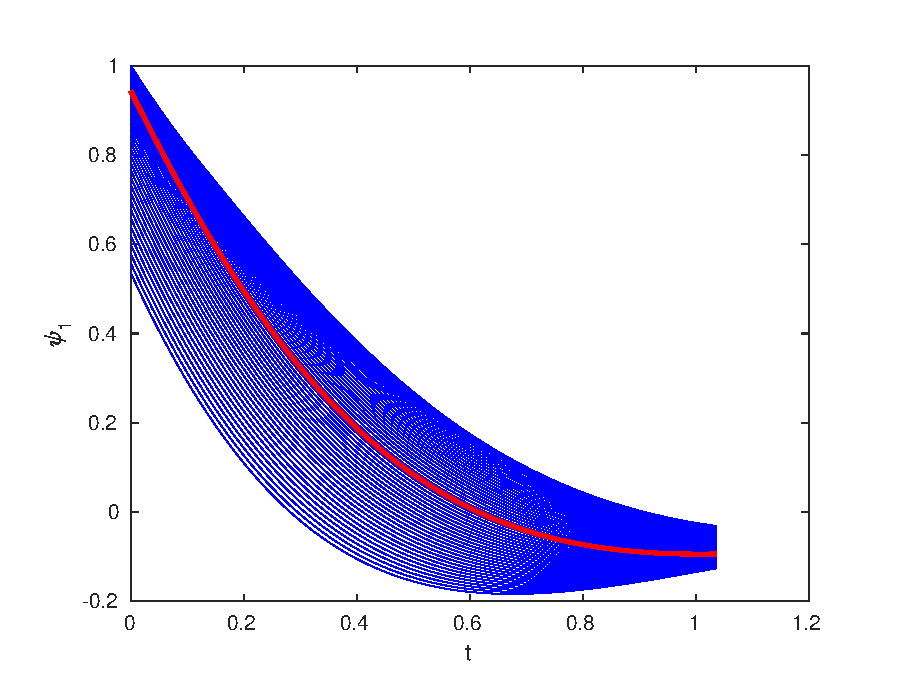
\includegraphics[width=45mm]{2tp1.eps}
	\hfill
	\caption{График $(t, \, \psi_1)$}
    \hfill
	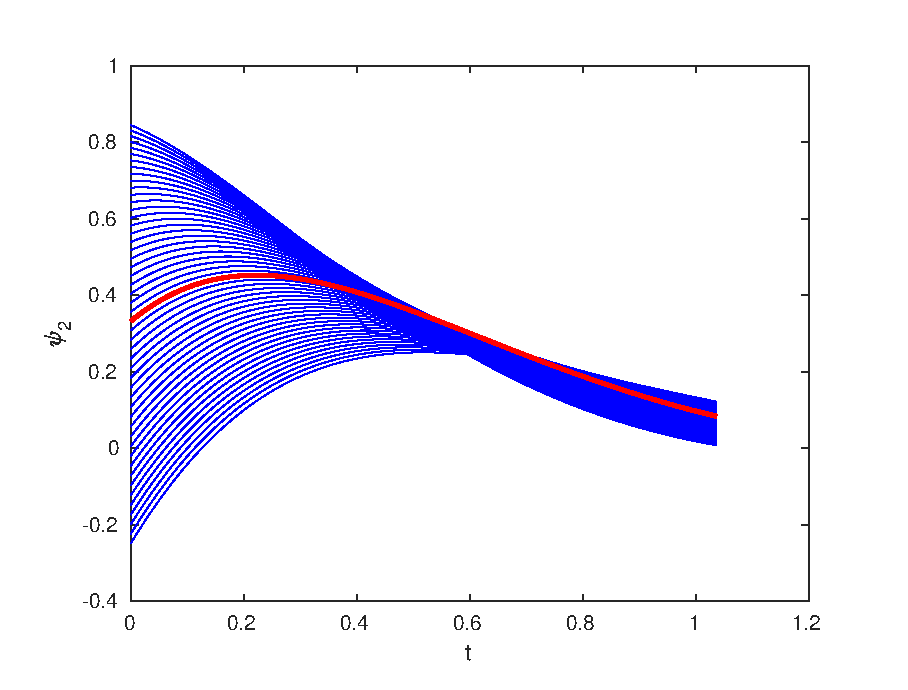
\includegraphics[width=45mm]{2tp2.eps}
	\hfill
	\caption{График $(t, \, \psi_2)$}
\end{multicols}
\end{figure}	

\newpage
\section{Разрывность зависимости $t_1$ от входных параметров}

\paragraph{Пример 1\\}
\begin{equation}
A = \begin{bmatrix}
0 & 3 \\ -3 & 0
\end{bmatrix},\ 
B = \begin{bmatrix}
1 & 0 \\ 0 & 1
\end{bmatrix}, \
f = \begin{bmatrix}
0 \\ 0
\end{bmatrix},
\end{equation}

$$\X_0 = \mathbb{B}\left(\Cl{0}{-2}, 1\right),$$
$$\X_1 = \Conv{\left(3 + \frac1{\sqrt{2}}\right)\Cl{1}{1}} + \mathbb{B}(0, 1),$$
$$\PS = \{u\colon u_1^2 + u_2^2 \le 1\}.$$

Центр координат является особой точкой типа неустойчивый фокус для матрицы $A$. При этом матрица
$A$ влияет на траекторию сильнее управления, и траектория не может выйти за пределы некоторой спирали.
При расположении терминального множества на крайней траектории оно будет достижимо за один оборот
вокруг центра координат, однако при сколь угодно малом увелечении координаты его центра на перемещение
потребуется уже два оборота, и значение функционала $t_1^*$ изменится скачком, то есть зависимость не
является непрерывной.

Первый рисунок соответствует поставленной задаче. Во втором случае
остаются неизменными все множества, кроме целевого, вместо которого рассматривается возмущенное 
$$ \tilde{\X_1} = \X_1 + \Cl{0.1}{0.1}.$$


\begin{figure}[h]
\begin{multicols}{2}
	\hfill
	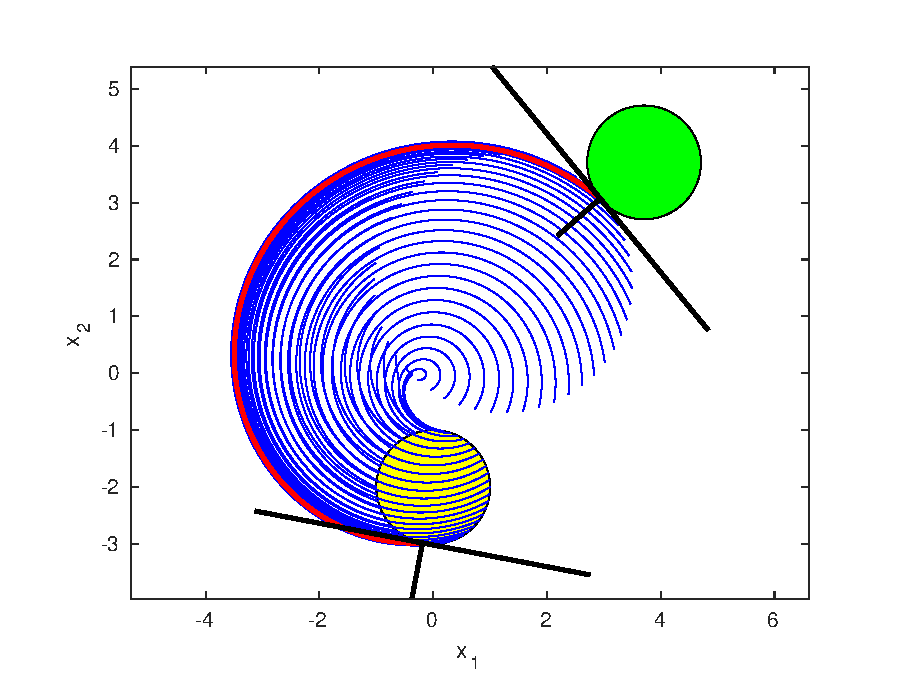
\includegraphics[width=80mm]{3_1.eps}
	\hfill
	\caption{$t_1^* = 1.2680$}
	\hfill
	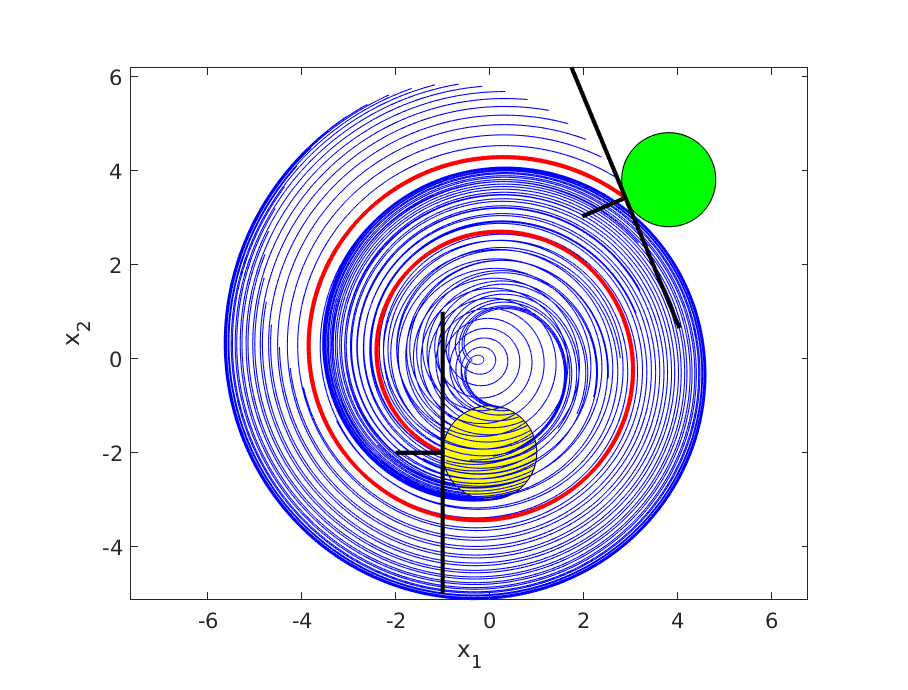
\includegraphics[width=80mm]{3_2.eps}
	\hfill
	\caption{$t_1^* = 3.0060$}
\end{multicols}
\end{figure}	

\paragraph{Пример 2\\}
\begin{equation}
A = \begin{bmatrix}
1 & 0 \\ 0 & 0
\end{bmatrix},\ 
B = \begin{bmatrix}
1 & 0 \\ 0 & 1
\end{bmatrix}, \
f = \begin{bmatrix}
-1 \\ 0
\end{bmatrix},
\end{equation}

$$\X_0 = \mathbb{B}\left(\Cl{-1}{0}, 1\right), $$
$$\X_1 = \Conv{\Cl{3}{0}} + \mathbb{B}(0, 1),$$
$$\PS = \{u\colon u_1^2 + u_2^2 \le 1\}.$$

Следующий пример показывает, что разрывы у функционала, вообще говоря, могут быть и второго рода.
Здесь все точки начального множества неположительны, а вектор $f$ <<тянет>> решение влево с единичной
скоростью. А так как управления ограничены единичным кругом, выйти в область $\{x_1 > 0\}$ в
этой задаче невозможно, то есть $t_1^* = +\infty$. Однако при сколь угодно малом смещении начального
множества вправо, появляется решение, выходящее из точки $\Cl{0}{1+\epsilon}$.
\begin{figure}[h]
\begin{multicols}{2}
	\hfill
	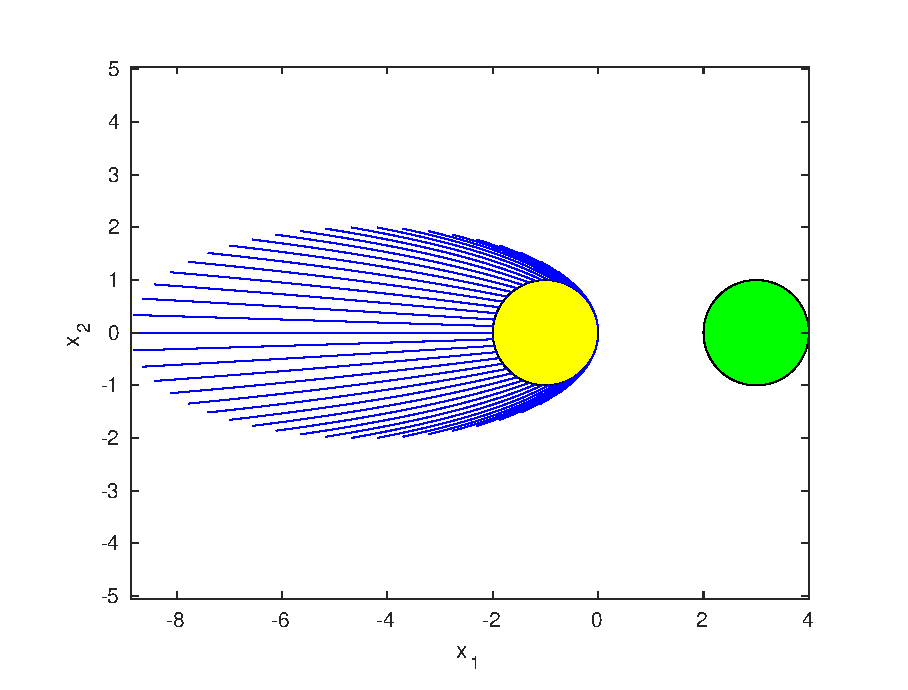
\includegraphics[width=80mm]{4_1.eps}
	\hfill
	\caption{$t_1^* = +\infty$}
	\hfill
	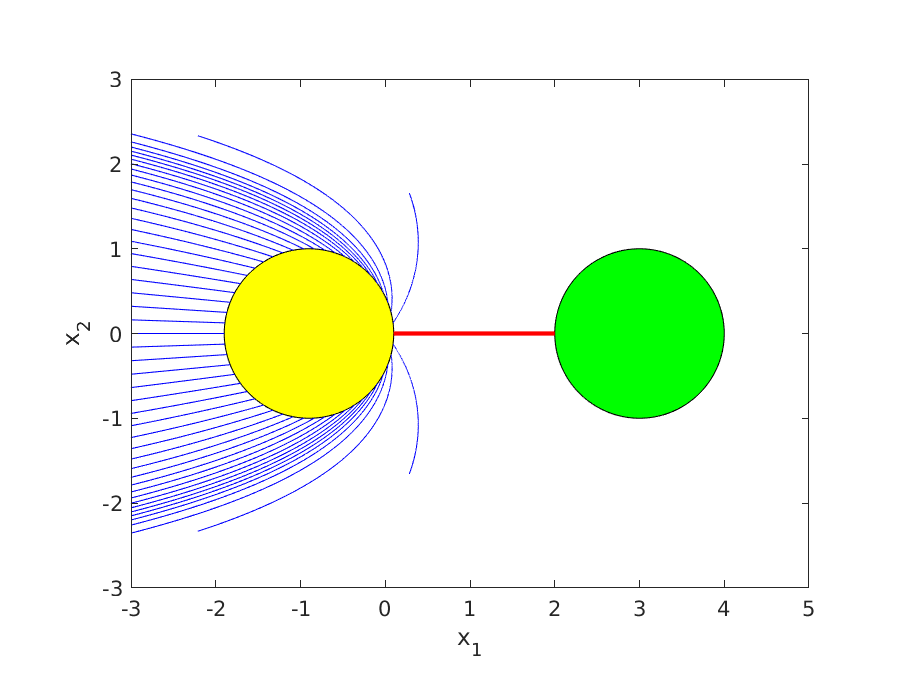
\includegraphics[width=80mm]{4_2.eps}
	\hfill
	\caption{$t_1^* = 2.9960$}
\end{multicols}
\end{figure}


\begin{thebibliography}{0}
\bibitem{rublev}
	Рублев~И.В. Лекции по оптимальному управлению. ВМК МГУ, 2019. 
\end{thebibliography}


\end{document}